\documentclass[twoside]{book}

% Packages required by doxygen
\usepackage{fixltx2e}
\usepackage{calc}
\usepackage{doxygen}
\usepackage[export]{adjustbox} % also loads graphicx
\usepackage{graphicx}
\usepackage[utf8]{inputenc}
\usepackage{makeidx}
\usepackage{multicol}
\usepackage{multirow}
\PassOptionsToPackage{warn}{textcomp}
\usepackage{textcomp}
\usepackage[nointegrals]{wasysym}
\usepackage[table]{xcolor}

% Font selection
\usepackage[T1]{fontenc}
\usepackage[scaled=.90]{helvet}
\usepackage{courier}
\usepackage{amssymb}
\usepackage{sectsty}
\renewcommand{\familydefault}{\sfdefault}
\allsectionsfont{%
  \fontseries{bc}\selectfont%
  \color{darkgray}%
}
\renewcommand{\DoxyLabelFont}{%
  \fontseries{bc}\selectfont%
  \color{darkgray}%
}
\newcommand{\+}{\discretionary{\mbox{\scriptsize$\hookleftarrow$}}{}{}}

% Page & text layout
\usepackage{geometry}
\geometry{%
  a4paper,%
  top=2.5cm,%
  bottom=2.5cm,%
  left=2.5cm,%
  right=2.5cm%
}
\tolerance=750
\hfuzz=15pt
\hbadness=750
\setlength{\emergencystretch}{15pt}
\setlength{\parindent}{0cm}
\setlength{\parskip}{3ex plus 2ex minus 2ex}
\makeatletter
\renewcommand{\paragraph}{%
  \@startsection{paragraph}{4}{0ex}{-1.0ex}{1.0ex}{%
    \normalfont\normalsize\bfseries\SS@parafont%
  }%
}
\renewcommand{\subparagraph}{%
  \@startsection{subparagraph}{5}{0ex}{-1.0ex}{1.0ex}{%
    \normalfont\normalsize\bfseries\SS@subparafont%
  }%
}
\makeatother

% Headers & footers
\usepackage{fancyhdr}
\pagestyle{fancyplain}
\fancyhead[LE]{\fancyplain{}{\bfseries\thepage}}
\fancyhead[CE]{\fancyplain{}{}}
\fancyhead[RE]{\fancyplain{}{\bfseries\leftmark}}
\fancyhead[LO]{\fancyplain{}{\bfseries\rightmark}}
\fancyhead[CO]{\fancyplain{}{}}
\fancyhead[RO]{\fancyplain{}{\bfseries\thepage}}
\fancyfoot[LE]{\fancyplain{}{}}
\fancyfoot[CE]{\fancyplain{}{}}
\fancyfoot[RE]{\fancyplain{}{\bfseries\scriptsize Generated by Doxygen }}
\fancyfoot[LO]{\fancyplain{}{\bfseries\scriptsize Generated by Doxygen }}
\fancyfoot[CO]{\fancyplain{}{}}
\fancyfoot[RO]{\fancyplain{}{}}
\renewcommand{\footrulewidth}{0.4pt}
\renewcommand{\chaptermark}[1]{%
  \markboth{#1}{}%
}
\renewcommand{\sectionmark}[1]{%
  \markright{\thesection\ #1}%
}

% Indices & bibliography
\usepackage{natbib}
\usepackage[titles]{tocloft}
\setcounter{tocdepth}{3}
\setcounter{secnumdepth}{5}
\makeindex

% Hyperlinks (required, but should be loaded last)
\usepackage{ifpdf}
\ifpdf
  \usepackage[pdftex,pagebackref=true]{hyperref}
\else
  \usepackage[ps2pdf,pagebackref=true]{hyperref}
\fi
\hypersetup{%
  colorlinks=true,%
  linkcolor=blue,%
  citecolor=blue,%
  unicode%
}

% Custom commands
\newcommand{\clearemptydoublepage}{%
  \newpage{\pagestyle{empty}\cleardoublepage}%
}

\usepackage{caption}
\captionsetup{labelsep=space,justification=centering,font={bf},singlelinecheck=off,skip=4pt,position=top}

%===== C O N T E N T S =====

\begin{document}

% Titlepage & ToC
\hypersetup{pageanchor=false,
             bookmarksnumbered=true,
             pdfencoding=unicode
            }
\pagenumbering{alph}
\begin{titlepage}
\vspace*{7cm}
\begin{center}%
{\Large C\+R\+AB \\[1ex]\large 1.\+2 }\\
\vspace*{1cm}
{\large Generated by Doxygen 1.8.13}\\
\end{center}
\end{titlepage}
\clearemptydoublepage
\pagenumbering{roman}
\tableofcontents
\clearemptydoublepage
\pagenumbering{arabic}
\hypersetup{pageanchor=true}

%--- Begin generated contents ---
\chapter{Namespace Index}
\section{Namespace List}
Here is a list of all documented namespaces with brief descriptions\+:\begin{DoxyCompactList}
\item\contentsline{section}{\hyperlink{namespace_ui}{Ui} }{\pageref{namespace_ui}}{}
\end{DoxyCompactList}

\chapter{Hierarchical Index}
\section{Class Hierarchy}
This inheritance list is sorted roughly, but not completely, alphabetically\+:\begin{DoxyCompactList}
\item \contentsline{section}{Borne}{\pageref{class_borne}}{}
\item \contentsline{section}{Maintenance}{\pageref{class_maintenance}}{}
\item \contentsline{section}{Passerelle}{\pageref{class_passerelle}}{}
\item Q\+Date\begin{DoxyCompactList}
\item \contentsline{section}{Date}{\pageref{class_date}}{}
\end{DoxyCompactList}
\item Q\+Main\+Window\begin{DoxyCompactList}
\item \contentsline{section}{Main\+Window}{\pageref{class_main_window}}{}
\end{DoxyCompactList}
\item Q\+Sql\+Query\begin{DoxyCompactList}
\item \contentsline{section}{jeu\+Enregistrement}{\pageref{classjeu_enregistrement}}{}
\end{DoxyCompactList}
\item \contentsline{section}{Station}{\pageref{class_station}}{}
\item \contentsline{section}{Technicien}{\pageref{class_technicien}}{}
\item \contentsline{section}{Type\+Borne}{\pageref{class_type_borne}}{}
\item \contentsline{section}{visite}{\pageref{classvisite}}{}
\end{DoxyCompactList}

\chapter{Class Index}
\section{Class List}
Here are the classes, structs, unions and interfaces with brief descriptions\+:\begin{DoxyCompactList}
\item\contentsline{section}{\hyperlink{class_borne}{Borne} \\*The \hyperlink{class_borne}{Borne} class Permet de connaitre les bornes à réviser et leur durée }{\pageref{class_borne}}{}
\item\contentsline{section}{\hyperlink{class_date}{Date} \\*The \hyperlink{class_date}{Date} class Permet de savoir la date afin de vérifier si il y aura besoin de maintenance ou non }{\pageref{class_date}}{}
\item\contentsline{section}{\hyperlink{classjeu_enregistrement}{jeu\+Enregistrement} }{\pageref{classjeu_enregistrement}}{}
\item\contentsline{section}{\hyperlink{class_maintenance}{Maintenance} \\*The \hyperlink{class_maintenance}{Maintenance} class Permet d\textquotesingle{}affecter chaque maintenance à faire à des techniciens }{\pageref{class_maintenance}}{}
\item\contentsline{section}{\hyperlink{class_main_window}{Main\+Window} }{\pageref{class_main_window}}{}
\item\contentsline{section}{\hyperlink{class_passerelle}{Passerelle} \\*The \hyperlink{class_passerelle}{Passerelle} class Permet d\textquotesingle{}effectuer toutes les requêtes sql }{\pageref{class_passerelle}}{}
\item\contentsline{section}{\hyperlink{class_station}{Station} \\*The \hyperlink{class_station}{Station} class Permet de savoir dans qu\textquotesingle{}elle sation il faut faire de la maintenance }{\pageref{class_station}}{}
\item\contentsline{section}{\hyperlink{class_technicien}{Technicien} \\*The \hyperlink{class_technicien}{Technicien} class Permet de récupérer les informations des techniciens afin de les affecter à des visites équitablement }{\pageref{class_technicien}}{}
\item\contentsline{section}{\hyperlink{class_type_borne}{Type\+Borne} \\*The \hyperlink{class_type_borne}{Type\+Borne} class Permet de référence les type de borne stocké dand la bdd }{\pageref{class_type_borne}}{}
\item\contentsline{section}{\hyperlink{classvisite}{visite} \\*The visite class Permet de référencé les visites à réaliser à partir de la base de données }{\pageref{classvisite}}{}
\end{DoxyCompactList}

\chapter{Namespace Documentation}
\hypertarget{namespace_ui}{}\section{Ui Namespace Reference}
\label{namespace_ui}\index{Ui@{Ui}}


\subsection{Detailed Description}
\begin{DoxyAuthor}{Author}
Mainard Jérémy 
\end{DoxyAuthor}
\begin{DoxyDate}{Date}
2019-\/11-\/20 
\end{DoxyDate}

\chapter{Class Documentation}
\hypertarget{class_borne}{}\section{Borne Class Reference}
\label{class_borne}\index{Borne@{Borne}}


The \hyperlink{class_borne}{Borne} class Permet de connaitre les bornes à réviser et leur durée.  




{\ttfamily \#include $<$borne.\+h$>$}

\subsection*{Public Member Functions}
\begin{DoxyCompactItemize}
\item 
\mbox{\Hypertarget{class_borne_aba0be924c6cb39fe8cdeffe27407fc3f}\label{class_borne_aba0be924c6cb39fe8cdeffe27407fc3f}} 
{\bfseries Borne} (int un\+Id\+Borne, \hyperlink{class_date}{Date} une\+Date\+Derniere\+Revision, int un\+Indice\+Compteur\+Unites, \hyperlink{class_type_borne}{Type\+Borne} un\+Type)
\item 
int \hyperlink{class_borne_aba8f90c81ef4efbe239e67e12015bb44}{get\+Duree\+Revision} ()
\begin{DoxyCompactList}\small\item\em \hyperlink{class_borne_aba8f90c81ef4efbe239e67e12015bb44}{Borne\+::get\+Duree\+Revision}. \end{DoxyCompactList}\item 
bool \hyperlink{class_borne_a40c1a1a990a10b8bc1421a1a39b7300a}{est\+A\+Reviser} ()
\begin{DoxyCompactList}\small\item\em \hyperlink{class_borne_a40c1a1a990a10b8bc1421a1a39b7300a}{Borne\+::est\+A\+Reviser}. \end{DoxyCompactList}\end{DoxyCompactItemize}


\subsection{Detailed Description}
The \hyperlink{class_borne}{Borne} class Permet de connaitre les bornes à réviser et leur durée. 

\subsection{Member Function Documentation}
\mbox{\Hypertarget{class_borne_a40c1a1a990a10b8bc1421a1a39b7300a}\label{class_borne_a40c1a1a990a10b8bc1421a1a39b7300a}} 
\index{Borne@{Borne}!est\+A\+Reviser@{est\+A\+Reviser}}
\index{est\+A\+Reviser@{est\+A\+Reviser}!Borne@{Borne}}
\subsubsection{\texorpdfstring{est\+A\+Reviser()}{estAReviser()}}
{\footnotesize\ttfamily bool Borne\+::est\+A\+Reviser (\begin{DoxyParamCaption}{ }\end{DoxyParamCaption})}



\hyperlink{class_borne_a40c1a1a990a10b8bc1421a1a39b7300a}{Borne\+::est\+A\+Reviser}. 

\begin{DoxyReturn}{Returns}
retourne si oui ou non la borne est à réviser Procédure permettant de savoir par un bool si la borne doit etre réviser en fonction du nombre de jour ou de ce qu\textquotesingle{}il y a eu de consommée en W\+A\+T\+TS. 
\end{DoxyReturn}
\mbox{\Hypertarget{class_borne_aba8f90c81ef4efbe239e67e12015bb44}\label{class_borne_aba8f90c81ef4efbe239e67e12015bb44}} 
\index{Borne@{Borne}!get\+Duree\+Revision@{get\+Duree\+Revision}}
\index{get\+Duree\+Revision@{get\+Duree\+Revision}!Borne@{Borne}}
\subsubsection{\texorpdfstring{get\+Duree\+Revision()}{getDureeRevision()}}
{\footnotesize\ttfamily int Borne\+::get\+Duree\+Revision (\begin{DoxyParamCaption}{ }\end{DoxyParamCaption})}



\hyperlink{class_borne_aba8f90c81ef4efbe239e67e12015bb44}{Borne\+::get\+Duree\+Revision}. 

\begin{DoxyReturn}{Returns}
retourne un int indiquant la durée de revision Procédure retournant la durée en minutes requise pour réaliser la révision sur la borne, cette durée étant fonction du type de la borne 
\end{DoxyReturn}


The documentation for this class was generated from the following files\+:\begin{DoxyCompactItemize}
\item 
borne.\+h\item 
borne.\+cpp\end{DoxyCompactItemize}

\hypertarget{class_date}{}\section{Date Class Reference}
\label{class_date}\index{Date@{Date}}


The \hyperlink{class_date}{Date} class Permet de savoir la date afin de vérifier si il y aura besoin de maintenance ou non.  




{\ttfamily \#include $<$date.\+h$>$}



Inheritance diagram for Date\+:\nopagebreak
\begin{figure}[H]
\begin{center}
\leavevmode
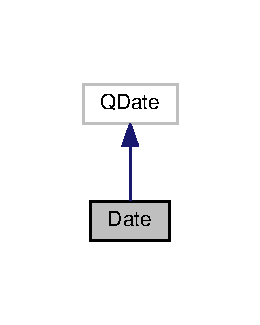
\includegraphics[width=125pt]{class_date__inherit__graph}
\end{center}
\end{figure}


Collaboration diagram for Date\+:\nopagebreak
\begin{figure}[H]
\begin{center}
\leavevmode
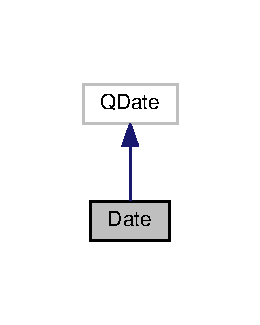
\includegraphics[width=125pt]{class_date__coll__graph}
\end{center}
\end{figure}
\subsection*{Public Member Functions}
\begin{DoxyCompactItemize}
\item 
\hyperlink{class_date_a2e0c4707435a4c3390e138b9ac6ee3f5}{Date} (int une\+Anne, int un\+Mois, int un\+Jour)
\begin{DoxyCompactList}\small\item\em Date\+::\+Date. \end{DoxyCompactList}\item 
int \hyperlink{class_date_a99c5677274bdaffadaedad4c888ccbca}{get\+Annee} ()
\begin{DoxyCompactList}\small\item\em \hyperlink{class_date_a99c5677274bdaffadaedad4c888ccbca}{Date\+::get\+Annee}. \end{DoxyCompactList}\item 
int \hyperlink{class_date_a6b16211abaa2c22418e82b8cd9d08bfe}{get\+Mois} ()
\begin{DoxyCompactList}\small\item\em \hyperlink{class_date_a6b16211abaa2c22418e82b8cd9d08bfe}{Date\+::get\+Mois}. \end{DoxyCompactList}\item 
int \hyperlink{class_date_a961e64bff2fdff7ee95bc335ca400d2f}{get\+Jour} ()
\begin{DoxyCompactList}\small\item\em \hyperlink{class_date_a961e64bff2fdff7ee95bc335ca400d2f}{Date\+::get\+Jour}. \end{DoxyCompactList}\item 
int \hyperlink{class_date_a45f1086b5028cdc71f7645f0a91d7731}{difference} (\hyperlink{class_date}{Date} une\+Date)
\begin{DoxyCompactList}\small\item\em \hyperlink{class_date_a45f1086b5028cdc71f7645f0a91d7731}{Date\+::difference}. \end{DoxyCompactList}\end{DoxyCompactItemize}
\subsection*{Static Public Member Functions}
\begin{DoxyCompactItemize}
\item 
static \hyperlink{class_date}{Date} \hyperlink{class_date_a4712c0d9ecfeb49472a847a905f62150}{aujourdhui} ()
\begin{DoxyCompactList}\small\item\em \hyperlink{class_date_a4712c0d9ecfeb49472a847a905f62150}{Date\+::aujourdhui}. \end{DoxyCompactList}\end{DoxyCompactItemize}


\subsection{Detailed Description}
The \hyperlink{class_date}{Date} class Permet de savoir la date afin de vérifier si il y aura besoin de maintenance ou non. 

\subsection{Constructor \& Destructor Documentation}
\mbox{\Hypertarget{class_date_a2e0c4707435a4c3390e138b9ac6ee3f5}\label{class_date_a2e0c4707435a4c3390e138b9ac6ee3f5}} 
\index{Date@{Date}!Date@{Date}}
\index{Date@{Date}!Date@{Date}}
\subsubsection{\texorpdfstring{Date()}{Date()}}
{\footnotesize\ttfamily Date\+::\+Date (\begin{DoxyParamCaption}\item[{int}]{une\+Anne,  }\item[{int}]{un\+Mois,  }\item[{int}]{un\+Jour }\end{DoxyParamCaption})}



Date\+::\+Date. 


\begin{DoxyParams}{Parameters}
{\em une\+Anne} & \\
\hline
{\em un\+Mois} & \\
\hline
{\em un\+Jour} & Constructeur permettant de récuperer la \hyperlink{class_date}{Date} du jour \\
\hline
\end{DoxyParams}


\subsection{Member Function Documentation}
\mbox{\Hypertarget{class_date_a4712c0d9ecfeb49472a847a905f62150}\label{class_date_a4712c0d9ecfeb49472a847a905f62150}} 
\index{Date@{Date}!aujourdhui@{aujourdhui}}
\index{aujourdhui@{aujourdhui}!Date@{Date}}
\subsubsection{\texorpdfstring{aujourdhui()}{aujourdhui()}}
{\footnotesize\ttfamily \hyperlink{class_date}{Date} Date\+::aujourdhui (\begin{DoxyParamCaption}{ }\end{DoxyParamCaption})\hspace{0.3cm}{\ttfamily [static]}}



\hyperlink{class_date_a4712c0d9ecfeb49472a847a905f62150}{Date\+::aujourdhui}. 

\begin{DoxyReturn}{Returns}
Retourne la date du jour Retourne la date du jour grace à la fonction Q\+Date sous forme Y\+Y-\/\+M\+M-\/\+D\+D\+DD 
\end{DoxyReturn}
\mbox{\Hypertarget{class_date_a45f1086b5028cdc71f7645f0a91d7731}\label{class_date_a45f1086b5028cdc71f7645f0a91d7731}} 
\index{Date@{Date}!difference@{difference}}
\index{difference@{difference}!Date@{Date}}
\subsubsection{\texorpdfstring{difference()}{difference()}}
{\footnotesize\ttfamily int Date\+::difference (\begin{DoxyParamCaption}\item[{\hyperlink{class_date}{Date}}]{une\+Date }\end{DoxyParamCaption})}



\hyperlink{class_date_a45f1086b5028cdc71f7645f0a91d7731}{Date\+::difference}. 


\begin{DoxyParams}{Parameters}
{\em une\+Date} & représente la date de la dernière revision de la borne \\
\hline
\end{DoxyParams}
\begin{DoxyReturn}{Returns}
retourne un int pour avoir une différence entre 2 jour Fonction permettant de savoir combien de jour /mois /année il y a de différence entre 2 date date à rentrer et une\+Date (\hyperlink{class_date}{Date} de révision ici) 
\end{DoxyReturn}
\mbox{\Hypertarget{class_date_a99c5677274bdaffadaedad4c888ccbca}\label{class_date_a99c5677274bdaffadaedad4c888ccbca}} 
\index{Date@{Date}!get\+Annee@{get\+Annee}}
\index{get\+Annee@{get\+Annee}!Date@{Date}}
\subsubsection{\texorpdfstring{get\+Annee()}{getAnnee()}}
{\footnotesize\ttfamily int Date\+::get\+Annee (\begin{DoxyParamCaption}{ }\end{DoxyParamCaption})}



\hyperlink{class_date_a99c5677274bdaffadaedad4c888ccbca}{Date\+::get\+Annee}. 

\begin{DoxyReturn}{Returns}
Retourne une variable int qui représente une année 
\end{DoxyReturn}
\mbox{\Hypertarget{class_date_a961e64bff2fdff7ee95bc335ca400d2f}\label{class_date_a961e64bff2fdff7ee95bc335ca400d2f}} 
\index{Date@{Date}!get\+Jour@{get\+Jour}}
\index{get\+Jour@{get\+Jour}!Date@{Date}}
\subsubsection{\texorpdfstring{get\+Jour()}{getJour()}}
{\footnotesize\ttfamily int Date\+::get\+Jour (\begin{DoxyParamCaption}{ }\end{DoxyParamCaption})}



\hyperlink{class_date_a961e64bff2fdff7ee95bc335ca400d2f}{Date\+::get\+Jour}. 

\begin{DoxyReturn}{Returns}
Retourne une variable int qui représente un Jour 
\end{DoxyReturn}
\mbox{\Hypertarget{class_date_a6b16211abaa2c22418e82b8cd9d08bfe}\label{class_date_a6b16211abaa2c22418e82b8cd9d08bfe}} 
\index{Date@{Date}!get\+Mois@{get\+Mois}}
\index{get\+Mois@{get\+Mois}!Date@{Date}}
\subsubsection{\texorpdfstring{get\+Mois()}{getMois()}}
{\footnotesize\ttfamily int Date\+::get\+Mois (\begin{DoxyParamCaption}{ }\end{DoxyParamCaption})}



\hyperlink{class_date_a6b16211abaa2c22418e82b8cd9d08bfe}{Date\+::get\+Mois}. 

\begin{DoxyReturn}{Returns}
Retourne une variable int qui représente un Mois 
\end{DoxyReturn}


The documentation for this class was generated from the following files\+:\begin{DoxyCompactItemize}
\item 
date.\+h\item 
date.\+cpp\end{DoxyCompactItemize}

\hypertarget{classjeu_enregistrement}{}\section{jeu\+Enregistrement Class Reference}
\label{classjeu_enregistrement}\index{jeu\+Enregistrement@{jeu\+Enregistrement}}


Inheritance diagram for jeu\+Enregistrement\+:\nopagebreak
\begin{figure}[H]
\begin{center}
\leavevmode
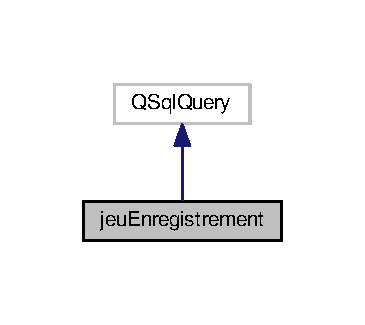
\includegraphics[width=175pt]{classjeu_enregistrement__inherit__graph}
\end{center}
\end{figure}


Collaboration diagram for jeu\+Enregistrement\+:\nopagebreak
\begin{figure}[H]
\begin{center}
\leavevmode
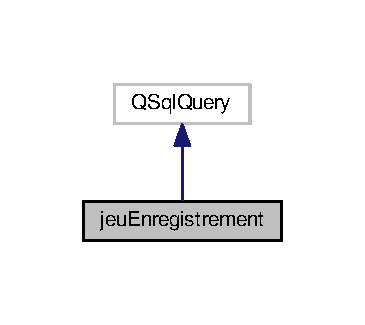
\includegraphics[width=175pt]{classjeu_enregistrement__coll__graph}
\end{center}
\end{figure}
\subsection*{Public Member Functions}
\begin{DoxyCompactItemize}
\item 
\mbox{\Hypertarget{classjeu_enregistrement_a941dbc3f9dd9c1c196ead81d045850bf}\label{classjeu_enregistrement_a941dbc3f9dd9c1c196ead81d045850bf}} 
{\bfseries jeu\+Enregistrement} (Q\+String la\+Requete)
\item 
\mbox{\Hypertarget{classjeu_enregistrement_aa26dd78c24b4fbaec948380d8907d4d9}\label{classjeu_enregistrement_aa26dd78c24b4fbaec948380d8907d4d9}} 
void \hyperlink{classjeu_enregistrement_aa26dd78c24b4fbaec948380d8907d4d9}{suivant} ()
\begin{DoxyCompactList}\small\item\em \hyperlink{classjeu_enregistrement_aa26dd78c24b4fbaec948380d8907d4d9}{jeu\+Enregistrement\+::suivant} Avance le curseur sur l\textquotesingle{}enregistrement suivant \end{DoxyCompactList}\item 
bool \hyperlink{classjeu_enregistrement_ad4689ab49e4a51fde86e3b00e15e473e}{fin\+Req} ()
\begin{DoxyCompactList}\small\item\em \hyperlink{classjeu_enregistrement_ad4689ab49e4a51fde86e3b00e15e473e}{jeu\+Enregistrement\+::fin\+Req} \end{DoxyCompactList}\item 
Q\+Variant \hyperlink{classjeu_enregistrement_acd8e0e1bc08d6b1a5c5966d565e134a2}{get\+Valeur} (Q\+String nom\+Champ)
\begin{DoxyCompactList}\small\item\em \hyperlink{classjeu_enregistrement_acd8e0e1bc08d6b1a5c5966d565e134a2}{jeu\+Enregistrement\+::get\+Valeur} \end{DoxyCompactList}\item 
\mbox{\Hypertarget{classjeu_enregistrement_adee0dc84769c49230dbd6b32ec0bd946}\label{classjeu_enregistrement_adee0dc84769c49230dbd6b32ec0bd946}} 
void \hyperlink{classjeu_enregistrement_adee0dc84769c49230dbd6b32ec0bd946}{fermer} ()
\begin{DoxyCompactList}\small\item\em \hyperlink{classjeu_enregistrement_adee0dc84769c49230dbd6b32ec0bd946}{jeu\+Enregistrement\+::fermer} Ferme le curseur et libère les ressources. \end{DoxyCompactList}\end{DoxyCompactItemize}


\subsection{Member Function Documentation}
\mbox{\Hypertarget{classjeu_enregistrement_ad4689ab49e4a51fde86e3b00e15e473e}\label{classjeu_enregistrement_ad4689ab49e4a51fde86e3b00e15e473e}} 
\index{jeu\+Enregistrement@{jeu\+Enregistrement}!fin\+Req@{fin\+Req}}
\index{fin\+Req@{fin\+Req}!jeu\+Enregistrement@{jeu\+Enregistrement}}
\subsubsection{\texorpdfstring{fin\+Req()}{finReq()}}
{\footnotesize\ttfamily bool jeu\+Enregistrement\+::fin\+Req (\begin{DoxyParamCaption}{ }\end{DoxyParamCaption})}



\hyperlink{classjeu_enregistrement_ad4689ab49e4a51fde86e3b00e15e473e}{jeu\+Enregistrement\+::fin\+Req} 

\begin{DoxyReturn}{Returns}
Un bool false or true si la requête est finie ou non 
\end{DoxyReturn}
\mbox{\Hypertarget{classjeu_enregistrement_acd8e0e1bc08d6b1a5c5966d565e134a2}\label{classjeu_enregistrement_acd8e0e1bc08d6b1a5c5966d565e134a2}} 
\index{jeu\+Enregistrement@{jeu\+Enregistrement}!get\+Valeur@{get\+Valeur}}
\index{get\+Valeur@{get\+Valeur}!jeu\+Enregistrement@{jeu\+Enregistrement}}
\subsubsection{\texorpdfstring{get\+Valeur()}{getValeur()}}
{\footnotesize\ttfamily Q\+Variant jeu\+Enregistrement\+::get\+Valeur (\begin{DoxyParamCaption}\item[{Q\+String}]{nom\+Champ }\end{DoxyParamCaption})}



\hyperlink{classjeu_enregistrement_acd8e0e1bc08d6b1a5c5966d565e134a2}{jeu\+Enregistrement\+::get\+Valeur} 


\begin{DoxyParams}{Parameters}
{\em nom\+Champ} & variable de S\+QL \\
\hline
\end{DoxyParams}
\begin{DoxyReturn}{Returns}
la valeur correspondant a nom\+Champ 
\end{DoxyReturn}


The documentation for this class was generated from the following files\+:\begin{DoxyCompactItemize}
\item 
jeuenregistrement.\+h\item 
jeuenregistrement.\+cpp\end{DoxyCompactItemize}

\hypertarget{class_maintenance}{}\section{Maintenance Class Reference}
\label{class_maintenance}\index{Maintenance@{Maintenance}}


The \hyperlink{class_maintenance}{Maintenance} class Permet d\textquotesingle{}affecter chaque maintenance à faire à des techniciens.  




{\ttfamily \#include $<$maintenance.\+h$>$}

\subsection*{Public Member Functions}
\begin{DoxyCompactItemize}
\item 
\mbox{\Hypertarget{class_maintenance_a8b51c17cc3e17405ce39fb2ec973df99}\label{class_maintenance_a8b51c17cc3e17405ce39fb2ec973df99}} 
\hyperlink{class_maintenance_a8b51c17cc3e17405ce39fb2ec973df99}{Maintenance} ()
\begin{DoxyCompactList}\small\item\em \hyperlink{class_maintenance_a8b51c17cc3e17405ce39fb2ec973df99}{Maintenance\+::\+Maintenance} Constructeur permettant de créer des vecteur qui ne sont plus vide afin de les utiliser dans les 2 porchaines procédures. \end{DoxyCompactList}\item 
\mbox{\Hypertarget{class_maintenance_a626bf6af87da611c75d0d83d1630dac1}\label{class_maintenance_a626bf6af87da611c75d0d83d1630dac1}} 
void \hyperlink{class_maintenance_a626bf6af87da611c75d0d83d1630dac1}{reviser} ()
\begin{DoxyCompactList}\small\item\em \hyperlink{class_maintenance_a626bf6af87da611c75d0d83d1630dac1}{Maintenance\+::reviser} Procédure permettant d\textquotesingle{}établir l\textquotesingle{}ensemble des visites à réaliser sur les stations. \end{DoxyCompactList}\item 
\mbox{\Hypertarget{class_maintenance_a1f6bef0a1a529beeaea5ab622f473782}\label{class_maintenance_a1f6bef0a1a529beeaea5ab622f473782}} 
void \hyperlink{class_maintenance_a1f6bef0a1a529beeaea5ab622f473782}{affecter\+Visites} ()
\begin{DoxyCompactList}\small\item\em \hyperlink{class_maintenance_a1f6bef0a1a529beeaea5ab622f473782}{Maintenance\+::affecter\+Visites} Affecte les visites à réaliser aux techniciens, en répartissant équitablement le travail entre les techniciens. Chaque visite est affectée au technicien le moins occupé en temps total de maintenance préventive. L\textquotesingle{}état de chaque visite doit alors être mis à jour. \end{DoxyCompactList}\item 
\mbox{\Hypertarget{class_maintenance_a68a453b1f48630a776c1f1b6605dd707}\label{class_maintenance_a68a453b1f48630a776c1f1b6605dd707}} 
void \hyperlink{class_maintenance_a68a453b1f48630a776c1f1b6605dd707}{afficher\+Tout} ()
\begin{DoxyCompactList}\small\item\em \hyperlink{class_maintenance_a68a453b1f48630a776c1f1b6605dd707}{Maintenance\+::afficher\+Tout}. \end{DoxyCompactList}\end{DoxyCompactItemize}


\subsection{Detailed Description}
The \hyperlink{class_maintenance}{Maintenance} class Permet d\textquotesingle{}affecter chaque maintenance à faire à des techniciens. 

The documentation for this class was generated from the following files\+:\begin{DoxyCompactItemize}
\item 
maintenance.\+h\item 
maintenance.\+cpp\end{DoxyCompactItemize}

\hypertarget{class_main_window}{}\section{Main\+Window Class Reference}
\label{class_main_window}\index{Main\+Window@{Main\+Window}}


Inheritance diagram for Main\+Window\+:\nopagebreak
\begin{figure}[H]
\begin{center}
\leavevmode
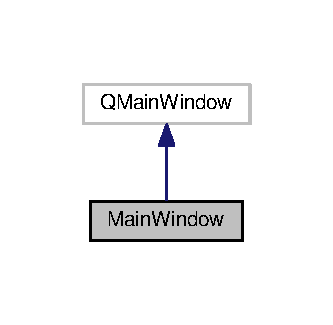
\includegraphics[width=160pt]{class_main_window__inherit__graph}
\end{center}
\end{figure}


Collaboration diagram for Main\+Window\+:\nopagebreak
\begin{figure}[H]
\begin{center}
\leavevmode
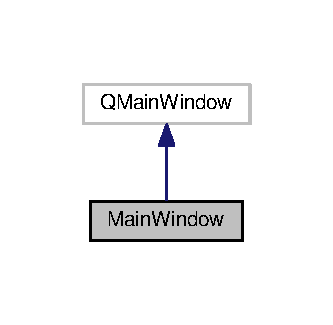
\includegraphics[width=160pt]{class_main_window__coll__graph}
\end{center}
\end{figure}
\subsection*{Public Member Functions}
\begin{DoxyCompactItemize}
\item 
\mbox{\Hypertarget{class_main_window_a8b244be8b7b7db1b08de2a2acb9409db}\label{class_main_window_a8b244be8b7b7db1b08de2a2acb9409db}} 
{\bfseries Main\+Window} (Q\+Widget $\ast$parent=0)
\end{DoxyCompactItemize}


The documentation for this class was generated from the following files\+:\begin{DoxyCompactItemize}
\item 
mainwindow.\+h\item 
mainwindow.\+cpp\end{DoxyCompactItemize}

\hypertarget{class_passerelle}{}\section{Passerelle Class Reference}
\label{class_passerelle}\index{Passerelle@{Passerelle}}


The \hyperlink{class_passerelle}{Passerelle} class Permet d\textquotesingle{}effectuer toutes les requêtes sql.  




{\ttfamily \#include $<$passerelle.\+h$>$}

\subsection*{Static Public Member Functions}
\begin{DoxyCompactItemize}
\item 
static Q\+Vector$<$ \hyperlink{class_technicien}{Technicien} $\ast$ $>$ \hyperlink{class_passerelle_a231a84d255da1885456f4637d4c88ee5}{charger\+Les\+Techniciens} ()
\begin{DoxyCompactList}\small\item\em \hyperlink{class_passerelle_a231a84d255da1885456f4637d4c88ee5}{Passerelle\+::charger\+Les\+Techniciens}. \end{DoxyCompactList}\item 
static Q\+Vector$<$ \hyperlink{class_borne}{Borne} $>$ \hyperlink{class_passerelle_a82347f95ecee56a567c080102c137ccd}{charger\+Les\+Bornes} (int un\+Id\+Station)
\begin{DoxyCompactList}\small\item\em \hyperlink{class_passerelle_a82347f95ecee56a567c080102c137ccd}{Passerelle\+::charger\+Les\+Bornes}. \end{DoxyCompactList}\item 
static Q\+Vector$<$ \hyperlink{class_station}{Station} $>$ \hyperlink{class_passerelle_a58f4340157dc6a2b5f720cf7ab09c980}{charger\+Les\+Stations} ()
\begin{DoxyCompactList}\small\item\em \hyperlink{class_passerelle_a58f4340157dc6a2b5f720cf7ab09c980}{Passerelle\+::charger\+Les\+Stations}. \end{DoxyCompactList}\item 
static void \hyperlink{class_passerelle_a82488527c9e08f60c905c0ec8a95187a}{enregistrer\+Visite} (\hyperlink{classvisite}{visite} une\+Visite, int mat\+Le\+Technicien, qint64 compteur\+Visite\+Id)
\begin{DoxyCompactList}\small\item\em \hyperlink{class_passerelle_a82488527c9e08f60c905c0ec8a95187a}{Passerelle\+::enregistrer\+Visite}. \end{DoxyCompactList}\end{DoxyCompactItemize}


\subsection{Detailed Description}
The \hyperlink{class_passerelle}{Passerelle} class Permet d\textquotesingle{}effectuer toutes les requêtes sql. 

\subsection{Member Function Documentation}
\mbox{\Hypertarget{class_passerelle_a82347f95ecee56a567c080102c137ccd}\label{class_passerelle_a82347f95ecee56a567c080102c137ccd}} 
\index{Passerelle@{Passerelle}!charger\+Les\+Bornes@{charger\+Les\+Bornes}}
\index{charger\+Les\+Bornes@{charger\+Les\+Bornes}!Passerelle@{Passerelle}}
\subsubsection{\texorpdfstring{charger\+Les\+Bornes()}{chargerLesBornes()}}
{\footnotesize\ttfamily Q\+Vector$<$ \hyperlink{class_borne}{Borne} $>$ Passerelle\+::charger\+Les\+Bornes (\begin{DoxyParamCaption}\item[{int}]{un\+Id\+Station }\end{DoxyParamCaption})\hspace{0.3cm}{\ttfamily [static]}}



\hyperlink{class_passerelle_a82347f95ecee56a567c080102c137ccd}{Passerelle\+::charger\+Les\+Bornes}. 

\begin{DoxyReturn}{Returns}
charges les bornes des stations dans un vecteur 
\end{DoxyReturn}
\mbox{\Hypertarget{class_passerelle_a58f4340157dc6a2b5f720cf7ab09c980}\label{class_passerelle_a58f4340157dc6a2b5f720cf7ab09c980}} 
\index{Passerelle@{Passerelle}!charger\+Les\+Stations@{charger\+Les\+Stations}}
\index{charger\+Les\+Stations@{charger\+Les\+Stations}!Passerelle@{Passerelle}}
\subsubsection{\texorpdfstring{charger\+Les\+Stations()}{chargerLesStations()}}
{\footnotesize\ttfamily Q\+Vector$<$ \hyperlink{class_station}{Station} $>$ Passerelle\+::charger\+Les\+Stations (\begin{DoxyParamCaption}{ }\end{DoxyParamCaption})\hspace{0.3cm}{\ttfamily [static]}}



\hyperlink{class_passerelle_a58f4340157dc6a2b5f720cf7ab09c980}{Passerelle\+::charger\+Les\+Stations}. 

\begin{DoxyReturn}{Returns}
charge les sations de la bdd 
\end{DoxyReturn}
\mbox{\Hypertarget{class_passerelle_a231a84d255da1885456f4637d4c88ee5}\label{class_passerelle_a231a84d255da1885456f4637d4c88ee5}} 
\index{Passerelle@{Passerelle}!charger\+Les\+Techniciens@{charger\+Les\+Techniciens}}
\index{charger\+Les\+Techniciens@{charger\+Les\+Techniciens}!Passerelle@{Passerelle}}
\subsubsection{\texorpdfstring{charger\+Les\+Techniciens()}{chargerLesTechniciens()}}
{\footnotesize\ttfamily Q\+Vector$<$ \hyperlink{class_technicien}{Technicien} $\ast$ $>$ Passerelle\+::charger\+Les\+Techniciens (\begin{DoxyParamCaption}{ }\end{DoxyParamCaption})\hspace{0.3cm}{\ttfamily [static]}}



\hyperlink{class_passerelle_a231a84d255da1885456f4637d4c88ee5}{Passerelle\+::charger\+Les\+Techniciens}. 

\begin{DoxyReturn}{Returns}
Charge les techniciens dans un vecteur 
\end{DoxyReturn}
\mbox{\Hypertarget{class_passerelle_a82488527c9e08f60c905c0ec8a95187a}\label{class_passerelle_a82488527c9e08f60c905c0ec8a95187a}} 
\index{Passerelle@{Passerelle}!enregistrer\+Visite@{enregistrer\+Visite}}
\index{enregistrer\+Visite@{enregistrer\+Visite}!Passerelle@{Passerelle}}
\subsubsection{\texorpdfstring{enregistrer\+Visite()}{enregistrerVisite()}}
{\footnotesize\ttfamily void Passerelle\+::enregistrer\+Visite (\begin{DoxyParamCaption}\item[{\hyperlink{classvisite}{visite}}]{une\+Visite,  }\item[{int}]{mat\+Le\+Technicien,  }\item[{qint64}]{compteur\+Visite\+Id }\end{DoxyParamCaption})\hspace{0.3cm}{\ttfamily [static]}}



\hyperlink{class_passerelle_a82488527c9e08f60c905c0ec8a95187a}{Passerelle\+::enregistrer\+Visite}. 


\begin{DoxyParams}{Parameters}
{\em une\+Visite} & \+: Vecteur des visites du technicien \\
\hline
{\em mat\+Le\+Technicien} & \+: Matricule du technicien \\
\hline
{\em compteur\+Visite\+Id} & \+: Id Visite Implémente les visites dans la bdd et créer un ID et les relie a techniciens et Bornes. \\
\hline
\end{DoxyParams}


The documentation for this class was generated from the following files\+:\begin{DoxyCompactItemize}
\item 
passerelle.\+h\item 
passerelle.\+cpp\end{DoxyCompactItemize}

\hypertarget{class_station}{}\section{Station Class Reference}
\label{class_station}\index{Station@{Station}}


The \hyperlink{class_station}{Station} class Permet de savoir dans qu\textquotesingle{}elle sation il faut faire de la maintenance.  




{\ttfamily \#include $<$station.\+h$>$}

\subsection*{Public Member Functions}
\begin{DoxyCompactItemize}
\item 
\mbox{\Hypertarget{class_station_ab3ce87c57bdf6c30fa057764a195c4a3}\label{class_station_ab3ce87c57bdf6c30fa057764a195c4a3}} 
{\bfseries Station} (int un\+Id\+Station, Q\+String un\+Libelle\+Emplacement, Q\+Vector$<$ \hyperlink{class_borne}{Borne} $>$ un\+Vecteur\+Borne)
\item 
int \hyperlink{class_station_a55b1b6e24c949165ca96d038125b72a6}{get\+Id} ()
\begin{DoxyCompactList}\small\item\em \hyperlink{class_station_a55b1b6e24c949165ca96d038125b72a6}{Station\+::get\+Id}. \end{DoxyCompactList}\item 
Q\+String \hyperlink{class_station_a6d4fa8bd0c2afa28aae831cd04938394}{get\+Libelle\+Emplacement} ()
\begin{DoxyCompactList}\small\item\em \hyperlink{class_station_a6d4fa8bd0c2afa28aae831cd04938394}{Station\+::get\+Libelle\+Emplacement}. \end{DoxyCompactList}\item 
\hyperlink{classvisite}{visite} $\ast$ \hyperlink{class_station_a0f0c47ed8e52e6d506c50512b915049a}{get\+Visite\+A\+Faire} ()
\begin{DoxyCompactList}\small\item\em \hyperlink{class_station_a0f0c47ed8e52e6d506c50512b915049a}{Station\+::get\+Visite\+A\+Faire}. \end{DoxyCompactList}\end{DoxyCompactItemize}


\subsection{Detailed Description}
The \hyperlink{class_station}{Station} class Permet de savoir dans qu\textquotesingle{}elle sation il faut faire de la maintenance. 

\subsection{Member Function Documentation}
\mbox{\Hypertarget{class_station_a55b1b6e24c949165ca96d038125b72a6}\label{class_station_a55b1b6e24c949165ca96d038125b72a6}} 
\index{Station@{Station}!get\+Id@{get\+Id}}
\index{get\+Id@{get\+Id}!Station@{Station}}
\subsubsection{\texorpdfstring{get\+Id()}{getId()}}
{\footnotesize\ttfamily int Station\+::get\+Id (\begin{DoxyParamCaption}{ }\end{DoxyParamCaption})}



\hyperlink{class_station_a55b1b6e24c949165ca96d038125b72a6}{Station\+::get\+Id}. 

\begin{DoxyReturn}{Returns}
retourne l\textquotesingle{}identifiant de la station Fonctions retournant l\textquotesingle{}identifiant de la \hyperlink{class_station}{Station} en int 
\end{DoxyReturn}
\mbox{\Hypertarget{class_station_a6d4fa8bd0c2afa28aae831cd04938394}\label{class_station_a6d4fa8bd0c2afa28aae831cd04938394}} 
\index{Station@{Station}!get\+Libelle\+Emplacement@{get\+Libelle\+Emplacement}}
\index{get\+Libelle\+Emplacement@{get\+Libelle\+Emplacement}!Station@{Station}}
\subsubsection{\texorpdfstring{get\+Libelle\+Emplacement()}{getLibelleEmplacement()}}
{\footnotesize\ttfamily Q\+String Station\+::get\+Libelle\+Emplacement (\begin{DoxyParamCaption}{ }\end{DoxyParamCaption})}



\hyperlink{class_station_a6d4fa8bd0c2afa28aae831cd04938394}{Station\+::get\+Libelle\+Emplacement}. 

\begin{DoxyReturn}{Returns}
retourne le libellé de l\textquotesingle{}emplacement Fonctions retournant les informations des Emplacements des Stations 
\end{DoxyReturn}
\mbox{\Hypertarget{class_station_a0f0c47ed8e52e6d506c50512b915049a}\label{class_station_a0f0c47ed8e52e6d506c50512b915049a}} 
\index{Station@{Station}!get\+Visite\+A\+Faire@{get\+Visite\+A\+Faire}}
\index{get\+Visite\+A\+Faire@{get\+Visite\+A\+Faire}!Station@{Station}}
\subsubsection{\texorpdfstring{get\+Visite\+A\+Faire()}{getVisiteAFaire()}}
{\footnotesize\ttfamily \hyperlink{classvisite}{visite} $\ast$ Station\+::get\+Visite\+A\+Faire (\begin{DoxyParamCaption}{ }\end{DoxyParamCaption})}



\hyperlink{class_station_a0f0c47ed8e52e6d506c50512b915049a}{Station\+::get\+Visite\+A\+Faire}. 

\begin{DoxyReturn}{Returns}
retourne une instance de classe Visite retourne une instance de classe Visite recensant toutes les bornes de la station qui nécessitent d\textquotesingle{}être révisées, ou null s\textquotesingle{}il n\textquotesingle{}y a aucune borne à réviser 
\end{DoxyReturn}


The documentation for this class was generated from the following files\+:\begin{DoxyCompactItemize}
\item 
station.\+h\item 
station.\+cpp\end{DoxyCompactItemize}

\hypertarget{class_technicien}{}\section{Technicien Class Reference}
\label{class_technicien}\index{Technicien@{Technicien}}


The \hyperlink{class_technicien}{Technicien} class Permet de récupérer les informations des techniciens afin de les affecter à des visites équitablement.  




{\ttfamily \#include $<$technicien.\+h$>$}

\subsection*{Public Member Functions}
\begin{DoxyCompactItemize}
\item 
\hyperlink{class_technicien_a2b13414c79a7a4f040522c34e0fd0aa6}{Technicien} (int un\+Matricule, Q\+String un\+Nom, Q\+String un\+Prenom)
\begin{DoxyCompactList}\small\item\em Technicien\+::\+Technicien. \end{DoxyCompactList}\item 
int \hyperlink{class_technicien_af111a0a23ae6ce1dbcb552817266744e}{get\+Temps\+Occupe} ()
\begin{DoxyCompactList}\small\item\em \hyperlink{class_technicien_af111a0a23ae6ce1dbcb552817266744e}{Technicien\+::get\+Temps\+Occupe}. \end{DoxyCompactList}\item 
void \hyperlink{class_technicien_ae214082b07ffa459ebfb99e9efd4da20}{affecter\+Visite} (\hyperlink{classvisite}{visite} $\ast$une\+Visite)
\begin{DoxyCompactList}\small\item\em \hyperlink{class_technicien_ae214082b07ffa459ebfb99e9efd4da20}{Technicien\+::affecter\+Visite}. \end{DoxyCompactList}\item 
Q\+Vector$<$ \hyperlink{classvisite}{visite} $\ast$ $>$ \hyperlink{class_technicien_a8ad18bf2c5758dbb6261594c544e47f9}{get\+Les\+Visites} ()
\begin{DoxyCompactList}\small\item\em \hyperlink{class_technicien_a8ad18bf2c5758dbb6261594c544e47f9}{Technicien\+::get\+Les\+Visites}. \end{DoxyCompactList}\item 
\mbox{\Hypertarget{class_technicien_a82c56619d7835292c0cfe48ceb05fa21}\label{class_technicien_a82c56619d7835292c0cfe48ceb05fa21}} 
Q\+String {\bfseries get\+Info} ()
\item 
\mbox{\Hypertarget{class_technicien_a6fe07be5429f9239023e4a8f551505ad}\label{class_technicien_a6fe07be5429f9239023e4a8f551505ad}} 
int {\bfseries get\+Matricule} ()
\end{DoxyCompactItemize}


\subsection{Detailed Description}
The \hyperlink{class_technicien}{Technicien} class Permet de récupérer les informations des techniciens afin de les affecter à des visites équitablement. 

\subsection{Constructor \& Destructor Documentation}
\mbox{\Hypertarget{class_technicien_a2b13414c79a7a4f040522c34e0fd0aa6}\label{class_technicien_a2b13414c79a7a4f040522c34e0fd0aa6}} 
\index{Technicien@{Technicien}!Technicien@{Technicien}}
\index{Technicien@{Technicien}!Technicien@{Technicien}}
\subsubsection{\texorpdfstring{Technicien()}{Technicien()}}
{\footnotesize\ttfamily Technicien\+::\+Technicien (\begin{DoxyParamCaption}\item[{int}]{un\+Matricule,  }\item[{Q\+String}]{un\+Nom,  }\item[{Q\+String}]{un\+Prenom }\end{DoxyParamCaption})}



Technicien\+::\+Technicien. 


\begin{DoxyParams}{Parameters}
{\em un\+Nom} & le nom du technicien \\
\hline
{\em un\+Prenom} & le prenom du technicien Constructeur permettant affecter des vistes au technicien pour le vecteur les\+Visites \\
\hline
\end{DoxyParams}


\subsection{Member Function Documentation}
\mbox{\Hypertarget{class_technicien_ae214082b07ffa459ebfb99e9efd4da20}\label{class_technicien_ae214082b07ffa459ebfb99e9efd4da20}} 
\index{Technicien@{Technicien}!affecter\+Visite@{affecter\+Visite}}
\index{affecter\+Visite@{affecter\+Visite}!Technicien@{Technicien}}
\subsubsection{\texorpdfstring{affecter\+Visite()}{affecterVisite()}}
{\footnotesize\ttfamily void Technicien\+::affecter\+Visite (\begin{DoxyParamCaption}\item[{\hyperlink{classvisite}{visite} $\ast$}]{une\+Visite }\end{DoxyParamCaption})}



\hyperlink{class_technicien_ae214082b07ffa459ebfb99e9efd4da20}{Technicien\+::affecter\+Visite}. 


\begin{DoxyParams}{Parameters}
{\em une\+Visite} & pointeur de visite afin de determiner de quelle visite on parle ajoute la visite une\+Visite dans les visites affectées au technicien \\
\hline
\end{DoxyParams}
\mbox{\Hypertarget{class_technicien_a8ad18bf2c5758dbb6261594c544e47f9}\label{class_technicien_a8ad18bf2c5758dbb6261594c544e47f9}} 
\index{Technicien@{Technicien}!get\+Les\+Visites@{get\+Les\+Visites}}
\index{get\+Les\+Visites@{get\+Les\+Visites}!Technicien@{Technicien}}
\subsubsection{\texorpdfstring{get\+Les\+Visites()}{getLesVisites()}}
{\footnotesize\ttfamily Q\+Vector$<$ \hyperlink{classvisite}{visite} $\ast$ $>$ Technicien\+::get\+Les\+Visites (\begin{DoxyParamCaption}{ }\end{DoxyParamCaption})}



\hyperlink{class_technicien_a8ad18bf2c5758dbb6261594c544e47f9}{Technicien\+::get\+Les\+Visites}. 

\begin{DoxyReturn}{Returns}
retourne l\textquotesingle{}ensemble des visites affectées au technicien Permet de savoir quel technicien a quel visites de programmé 
\end{DoxyReturn}
\mbox{\Hypertarget{class_technicien_af111a0a23ae6ce1dbcb552817266744e}\label{class_technicien_af111a0a23ae6ce1dbcb552817266744e}} 
\index{Technicien@{Technicien}!get\+Temps\+Occupe@{get\+Temps\+Occupe}}
\index{get\+Temps\+Occupe@{get\+Temps\+Occupe}!Technicien@{Technicien}}
\subsubsection{\texorpdfstring{get\+Temps\+Occupe()}{getTempsOccupe()}}
{\footnotesize\ttfamily int Technicien\+::get\+Temps\+Occupe (\begin{DoxyParamCaption}{ }\end{DoxyParamCaption})}



\hyperlink{class_technicien_af111a0a23ae6ce1dbcb552817266744e}{Technicien\+::get\+Temps\+Occupe}. 

\begin{DoxyReturn}{Returns}
Retourne la durée totale en minutes des visites affectées au technicien 
\end{DoxyReturn}


The documentation for this class was generated from the following files\+:\begin{DoxyCompactItemize}
\item 
technicien.\+h\item 
technicien.\+cpp\end{DoxyCompactItemize}

\hypertarget{class_type_borne}{}\section{Type\+Borne Class Reference}
\label{class_type_borne}\index{Type\+Borne@{Type\+Borne}}


The \hyperlink{class_type_borne}{Type\+Borne} class Permet de référence les type de borne stocké dand la bdd.  




{\ttfamily \#include $<$typeborne.\+h$>$}

\subsection*{Public Member Functions}
\begin{DoxyCompactItemize}
\item 
\mbox{\Hypertarget{class_type_borne_a32f9c836b0f0b34e86a53520a8f23674}\label{class_type_borne_a32f9c836b0f0b34e86a53520a8f23674}} 
{\bfseries Type\+Borne} (Q\+String un\+Code\+Type\+Borne, int une\+Duree\+Revision, int un\+Nb\+Jours\+Entre\+Revisions, int un\+Nb\+Unite\+Entre\+Revisions)
\item 
int \hyperlink{class_type_borne_aee58fc4a65b54cf00376c72df39ac0d9}{get\+Duree\+Revision} ()
\begin{DoxyCompactList}\small\item\em \hyperlink{class_type_borne_aee58fc4a65b54cf00376c72df39ac0d9}{Type\+Borne\+::get\+Duree\+Revision}. \end{DoxyCompactList}\item 
int \hyperlink{class_type_borne_a4921b40e0c20ec1c98ea167cb787e605}{get\+Nb\+Jours\+Entre\+Revisions} ()
\begin{DoxyCompactList}\small\item\em \hyperlink{class_type_borne_a4921b40e0c20ec1c98ea167cb787e605}{Type\+Borne\+::get\+Nb\+Jours\+Entre\+Revisions}. \end{DoxyCompactList}\item 
int \hyperlink{class_type_borne_aa99a6c098973997a77699bea1244a94f}{get\+Nb\+Unites\+Entre\+Revisions} ()
\begin{DoxyCompactList}\small\item\em \hyperlink{class_type_borne_aa99a6c098973997a77699bea1244a94f}{Type\+Borne\+::get\+Nb\+Unites\+Entre\+Revisions}. \end{DoxyCompactList}\end{DoxyCompactItemize}


\subsection{Detailed Description}
The \hyperlink{class_type_borne}{Type\+Borne} class Permet de référence les type de borne stocké dand la bdd. 

\subsection{Member Function Documentation}
\mbox{\Hypertarget{class_type_borne_aee58fc4a65b54cf00376c72df39ac0d9}\label{class_type_borne_aee58fc4a65b54cf00376c72df39ac0d9}} 
\index{Type\+Borne@{Type\+Borne}!get\+Duree\+Revision@{get\+Duree\+Revision}}
\index{get\+Duree\+Revision@{get\+Duree\+Revision}!Type\+Borne@{Type\+Borne}}
\subsubsection{\texorpdfstring{get\+Duree\+Revision()}{getDureeRevision()}}
{\footnotesize\ttfamily int Type\+Borne\+::get\+Duree\+Revision (\begin{DoxyParamCaption}{ }\end{DoxyParamCaption})}



\hyperlink{class_type_borne_aee58fc4a65b54cf00376c72df39ac0d9}{Type\+Borne\+::get\+Duree\+Revision}. 

\begin{DoxyReturn}{Returns}
un int qui correspond à la durée standard de révision d\textquotesingle{}une borne de ce type Retourne la durée en minutes requise pour réaliser la révision sur les bornes de ce type 
\end{DoxyReturn}
\mbox{\Hypertarget{class_type_borne_a4921b40e0c20ec1c98ea167cb787e605}\label{class_type_borne_a4921b40e0c20ec1c98ea167cb787e605}} 
\index{Type\+Borne@{Type\+Borne}!get\+Nb\+Jours\+Entre\+Revisions@{get\+Nb\+Jours\+Entre\+Revisions}}
\index{get\+Nb\+Jours\+Entre\+Revisions@{get\+Nb\+Jours\+Entre\+Revisions}!Type\+Borne@{Type\+Borne}}
\subsubsection{\texorpdfstring{get\+Nb\+Jours\+Entre\+Revisions()}{getNbJoursEntreRevisions()}}
{\footnotesize\ttfamily int Type\+Borne\+::get\+Nb\+Jours\+Entre\+Revisions (\begin{DoxyParamCaption}{ }\end{DoxyParamCaption})}



\hyperlink{class_type_borne_a4921b40e0c20ec1c98ea167cb787e605}{Type\+Borne\+::get\+Nb\+Jours\+Entre\+Revisions}. 

\begin{DoxyReturn}{Returns}
un int du nb de jour qu\textquotesingle{}il faut entre 2 révisions retourne le nombre de jours au-\/delà duquel il faut envisager une révision sur les bornes de ce type 
\end{DoxyReturn}
\mbox{\Hypertarget{class_type_borne_aa99a6c098973997a77699bea1244a94f}\label{class_type_borne_aa99a6c098973997a77699bea1244a94f}} 
\index{Type\+Borne@{Type\+Borne}!get\+Nb\+Unites\+Entre\+Revisions@{get\+Nb\+Unites\+Entre\+Revisions}}
\index{get\+Nb\+Unites\+Entre\+Revisions@{get\+Nb\+Unites\+Entre\+Revisions}!Type\+Borne@{Type\+Borne}}
\subsubsection{\texorpdfstring{get\+Nb\+Unites\+Entre\+Revisions()}{getNbUnitesEntreRevisions()}}
{\footnotesize\ttfamily int Type\+Borne\+::get\+Nb\+Unites\+Entre\+Revisions (\begin{DoxyParamCaption}{ }\end{DoxyParamCaption})}



\hyperlink{class_type_borne_aa99a6c098973997a77699bea1244a94f}{Type\+Borne\+::get\+Nb\+Unites\+Entre\+Revisions}. 

\begin{DoxyReturn}{Returns}
Retourne le nombre d\textquotesingle{}unités de recharge au-\/delà duquel il faut envisager une révision sur les bornes de ce type 
\end{DoxyReturn}


The documentation for this class was generated from the following files\+:\begin{DoxyCompactItemize}
\item 
typeborne.\+h\item 
typeborne.\+cpp\end{DoxyCompactItemize}

\hypertarget{classvisite}{}\section{visite Class Reference}
\label{classvisite}\index{visite@{visite}}


The visite class Permet de référencé les visites à réaliser à partir de la base de données.  




{\ttfamily \#include $<$visite.\+h$>$}

\subsection*{Public Member Functions}
\begin{DoxyCompactItemize}
\item 
\hyperlink{classvisite_a197936c1244f7c9fd0a2eca7038533f9}{visite} (Q\+Vector$<$ \hyperlink{class_borne}{Borne} $>$ les\+Bornes\+A\+Visiter, \hyperlink{class_station}{Station} $\ast$une\+Station)
\begin{DoxyCompactList}\small\item\em visite\+::visite \end{DoxyCompactList}\item 
int \hyperlink{classvisite_a608738dbddc358c0805228e0aac5818c}{get\+Duree\+Totale} ()
\begin{DoxyCompactList}\small\item\em \hyperlink{classvisite_a608738dbddc358c0805228e0aac5818c}{visite\+::get\+Duree\+Totale} \end{DoxyCompactList}\item 
char \hyperlink{classvisite_a6da950d2a01048158c7abcc1ebdfec22}{get\+Etat} ()
\begin{DoxyCompactList}\small\item\em \hyperlink{classvisite_a6da950d2a01048158c7abcc1ebdfec22}{visite\+::get\+Etat} \end{DoxyCompactList}\item 
\mbox{\Hypertarget{classvisite_a731243b15c082ddff3294c09524c39e4}\label{classvisite_a731243b15c082ddff3294c09524c39e4}} 
void \hyperlink{classvisite_a731243b15c082ddff3294c09524c39e4}{changer\+Etat} ()
\begin{DoxyCompactList}\small\item\em \hyperlink{classvisite_a731243b15c082ddff3294c09524c39e4}{visite\+::changer\+Etat} Procédure modifiant l\textquotesingle{}état de la visite, de \textquotesingle{}p\textquotesingle{} programmée à \textquotesingle{}a\textquotesingle{} affectée, ou de \textquotesingle{}a\textquotesingle{} affectée à \textquotesingle{}r\textquotesingle{} réalisé \end{DoxyCompactList}\item 
Q\+String \hyperlink{classvisite_a7a948dd8b5c805a1f2a7d62c9268cb97}{get\+Info\+Visite} ()
\begin{DoxyCompactList}\small\item\em Visite\+::get\+Info Fonction qui renvoie les informations d\textquotesingle{}une visite. \end{DoxyCompactList}\end{DoxyCompactItemize}


\subsection{Detailed Description}
The visite class Permet de référencé les visites à réaliser à partir de la base de données. 

\subsection{Constructor \& Destructor Documentation}
\mbox{\Hypertarget{classvisite_a197936c1244f7c9fd0a2eca7038533f9}\label{classvisite_a197936c1244f7c9fd0a2eca7038533f9}} 
\index{visite@{visite}!visite@{visite}}
\index{visite@{visite}!visite@{visite}}
\subsubsection{\texorpdfstring{visite()}{visite()}}
{\footnotesize\ttfamily visite\+::visite (\begin{DoxyParamCaption}\item[{Q\+Vector$<$ \hyperlink{class_borne}{Borne} $>$}]{les\+Bornes\+A\+Visiter,  }\item[{\hyperlink{class_station}{Station} $\ast$}]{une\+Station }\end{DoxyParamCaption})}



visite\+::visite 


\begin{DoxyParams}{Parameters}
{\em les\+Bornes\+A\+Visiter} & vecteur recensant les bornes à visiter \\
\hline
{\em une\+Station} & station sur lesquelle le vetuer ce base pour savoir quelle borne est à visiter ce constructeur valorise tous les attributs privés de la classe Visite, y compris l\textquotesingle{}état et la durée totale de la visite \\
\hline
\end{DoxyParams}


\subsection{Member Function Documentation}
\mbox{\Hypertarget{classvisite_a608738dbddc358c0805228e0aac5818c}\label{classvisite_a608738dbddc358c0805228e0aac5818c}} 
\index{visite@{visite}!get\+Duree\+Totale@{get\+Duree\+Totale}}
\index{get\+Duree\+Totale@{get\+Duree\+Totale}!visite@{visite}}
\subsubsection{\texorpdfstring{get\+Duree\+Totale()}{getDureeTotale()}}
{\footnotesize\ttfamily int visite\+::get\+Duree\+Totale (\begin{DoxyParamCaption}{ }\end{DoxyParamCaption})}



\hyperlink{classvisite_a608738dbddc358c0805228e0aac5818c}{visite\+::get\+Duree\+Totale} 

\begin{DoxyReturn}{Returns}
Fonction retournant la durée totale en minutes requise pour réaliser l\textquotesingle{}ensemble des révisions prévues sur les bornes de la station 
\end{DoxyReturn}
\mbox{\Hypertarget{classvisite_a6da950d2a01048158c7abcc1ebdfec22}\label{classvisite_a6da950d2a01048158c7abcc1ebdfec22}} 
\index{visite@{visite}!get\+Etat@{get\+Etat}}
\index{get\+Etat@{get\+Etat}!visite@{visite}}
\subsubsection{\texorpdfstring{get\+Etat()}{getEtat()}}
{\footnotesize\ttfamily char visite\+::get\+Etat (\begin{DoxyParamCaption}{ }\end{DoxyParamCaption})}



\hyperlink{classvisite_a6da950d2a01048158c7abcc1ebdfec22}{visite\+::get\+Etat} 

\begin{DoxyReturn}{Returns}
retourne l\textquotesingle{}état de la visite Soit il retourne si oui ou non la visite à était fait 
\end{DoxyReturn}
\mbox{\Hypertarget{classvisite_a7a948dd8b5c805a1f2a7d62c9268cb97}\label{classvisite_a7a948dd8b5c805a1f2a7d62c9268cb97}} 
\index{visite@{visite}!get\+Info\+Visite@{get\+Info\+Visite}}
\index{get\+Info\+Visite@{get\+Info\+Visite}!visite@{visite}}
\subsubsection{\texorpdfstring{get\+Info\+Visite()}{getInfoVisite()}}
{\footnotesize\ttfamily Q\+String visite\+::get\+Info\+Visite (\begin{DoxyParamCaption}{ }\end{DoxyParamCaption})}



Visite\+::get\+Info Fonction qui renvoie les informations d\textquotesingle{}une visite. 

\begin{DoxyReturn}{Returns}
Chaine(\+Q\+String) \+: information au format texte de la visite (Etat,Durée,\hyperlink{class_station}{Station}) 
\end{DoxyReturn}


The documentation for this class was generated from the following files\+:\begin{DoxyCompactItemize}
\item 
visite.\+h\item 
visite.\+cpp\end{DoxyCompactItemize}

%--- End generated contents ---

% Index
\backmatter
\newpage
\phantomsection
\clearemptydoublepage
\addcontentsline{toc}{chapter}{Index}
\printindex

\end{document}
